\subsection{同型}
	圏論では射の等しさを表すときには等号を使うが、対象に対しての等号は制約が多い。そのため\textbf{同型}と呼ばれる同値関係を代わりに用いる。
	\begin{define}[同型]
		ある対象$A$と$B$が同型、つまり$A\cong B$であるとは、$i\circ i^{-1}=id_B$と$i^{-1}\circ i=id_A$を満たすようなある二つの射$\mor{i}{A}{B}$とその逆射$\mor{i^{-1}}{B}{A}$が存在するときである。このような射$i,i^{-1}$を\textbf{同型射}と呼ぶ。またこの時、$A$から$B$への射はすべてが同型射である必要はない。また、
	\end{define}
	\begin{center}
		\begin{tikzpicture}[auto]
			\node (a) at (-4, -1) {$A$};
			\node (b) at (-2, -1) {$B$};
			\draw[->,transform canvas={yshift=-3pt}] (a) to node[swap] {$i$}(b);
			\draw[->,transform canvas={yshift=3pt}] (b) to node[swap] {$i^{-1}$}(a);

			\node (a) at (0, 0) {$A$};
			\node (b) at (2, 0) {$B$};
			\node (b') at (0, -2) {$B$};
			\draw[->] (a) to node[swap] {$i$}(b');
			\draw[->] (b) to node {$id_B$}(b');
			\draw[->] (b) to node[swap] {$i^{-1}$}(a);

			\node (a) at (4, 0) {$B$};
			\node (b) at (6, 0) {$A$};
			\node (b') at (4, -2) {$A$};
			\draw[->] (a) to node[swap] {$i^{-1}$}(b');
			\draw[->] (b) to node {$id_A$}(b');
			\draw[->] (b) to node[swap] {$i$}(a);
		\end{tikzpicture}
	\end{center}
	同型は対象同士の相互互換のような関係性を表しているように思える。
  \begin{prop}
    同型は同値関係である。すなわち反射律、対称律、推移律を満たす。
  \end{prop}
  \begin{proof}~
    \begin{quote}
			\begin{mydescription}
				\item[反射律] 任意の対象$A$で$A\cong A$が成り立つことを証明すれば良い。$\mor{id_A}{A}{A}$を同型射とその逆射$(id_A)^{-1}$をまた$id_A$とすると、\[id_A\circ id_A = id_A,\,id_A\circ id_A = id_A\]が成り立つから、$id_A$は同型射であり$A\cong A$である。

				\item[対称律] 同型$A\cong B\Longrightarrow B\cong A$を示せば良い。同型$A\cong B$が同型射$\mor{i}{A}{B}$とその逆射$\mor{i^{-1}}{B}{A}$によって成り立つとする。この時、$i^{-1}$の逆射を$i$とみなすと、$i^{-1}\circ i=id_A$と$i\circ i^{-1}=id_B$が成り立つから、$B\cong A$となる。
				\item[推移律] $A\cong B,B\cong C\Longrightarrow A\cong C$を示せば良い。$A\cong B$の同型射を$\mor{i}{A}{B}$、$\mor{i^{-1}}{B}{A}$、$B\cong C$の同型射を$\mor{j}{B}{C}$、$\mor{j^{-1}}{C}{B}$とする。この時、$j\circ i$と$i^{-1}\circ j^{-1}$が同型射になることを示せば良い。
        \begin{center}
          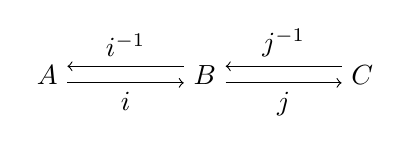
\begin{tikzpicture}[auto]
            \node (a) at (0, 0) {$A$};
            \node (b) at (2, 0) {$B$};
            \node (c) at (4, 0) {$C$};
            \draw[->,transform canvas={yshift=-3pt}] (a) to node[swap] {$i$}(b);
            \draw[->,transform canvas={yshift=3pt}] (b) to node[swap] {$i^{-1}$}(a);

            \draw[->,transform canvas={yshift=-3pt}] (b) to node[swap] {$j$}(c);
            \draw[->,transform canvas={yshift=3pt}] (c) to node[swap] {$j^{-1}$}(b);
          \end{tikzpicture}
        \end{center} 
				\begin{align*}
          (j\circ i)\circ (i^{-1}\circ j^{-1})&=j\circ(i\circ i^{-1})\circ j^{-1}&\text{(結合則)}\\
          &=j\circ(id_B)\circ j^{-1}&\text{(同型射の定義)}\\
          &=j\circ j^{-1}&\text{(恒等射の性質)}\\
          &=id_C&\text{(同型射の定義)}\\
          (i^{-1}\circ j^{-1})\circ(j\circ i)&=i^{-1}\circ(j^{-1}\circ j)\circ i&\text{(結合則)}\\
          &=i^{-1}\circ(id_B)\circ i&\text{(同型射の定義)}\\
          &=i^{-1}\circ i&\text{(恒等射の性質)}\\
          &=id_A&\text{(同型射の定義)}\\
        \end{align*}
        よって$j\circ i$と$i^{-1}\circ j^{-1}$は同型射となり、$A\cong C$が成り立つ。
      \end{mydescription}
    \end{quote}
  \end{proof}

  \begin{prop}[同型と元]
    同型$A\cong B$で、$\mor{i}{A}{B}$が同型射である時、
    \[i(a)=b\iff i^{-1}(b)=a\]であり、この時$a\sim b$とする。そしてこのような$a,b$の対応は\textbf{一対一対応}である。\\
    すなわち、$a$に対して$a\sim b$となるような$b$は\textbf{一意}に\textbf{存在}する。
    \begin{center}
      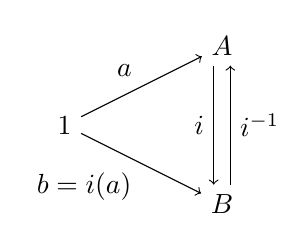
\begin{tikzpicture}[auto]
        \node (1) at (-2, 1) {$1$};
        \node (a) at (0, 2) {$A$};
        \node (b) at (0, 0) {$B$};
        \draw[->] (1) to node{$a$}(a);
        \draw[->] (1) to node[swap]{$b=i(a)$}(b);
        \draw[->,transform canvas={xshift=-3pt}] (a) to node[swap] {$i$}(b);
        \draw[->,transform canvas={xshift=3pt}] (b) to node[swap] {$i^{-1}$}(a);
      \end{tikzpicture}
    \end{center} 
  \end{prop}
  \begin{proof}
    $(\Longrightarrow)$を示す。
    \begin{align*}
      i(a)&=b\\
      i^{-1}(i(a))&=i^{-1}(b)\\
      (i^{-1}\circ i)(a)&=i^{-1}(b)&\text{(写像の合成の定義)}\\
      id_A(a)&=i^{-1}(b)&\text{(同型射の定義)}\\
      a &=i^{-1}(b)&\text{(恒等射の定義)}
    \end{align*}
    同様に$(\Longleftarrow)$も示せるから$i(a)=b\iff i^{-1}(b)=a$である。\\
    $a$に対して$a\sim b$なる$b$が存在することは、写像$\mor{i}{A}{B}$の全域性から分かる。すなわち$a\sim i(a)$である。次に$b$の一意性を示す。
    $a\sim b,\ a\sim b'$とする。この時$b=b'$を示せばよい。
    \begin{align*}
      i^{-1}(b')&=a&\text{($a\sim b'$の定義)}\\
      i(i^{-1}(b'))&=i(a)\\
      id_B(b')&=i(a)&\text{(写像の合成の定義と同型射の定義)}\\
      b'&=i(a)&\text{(恒等射の定義)}\\
      b'&=b&\text{($a\sim b$の定義)}
    \end{align*}
    よって$b$が一意に定まることが分かり、$a,b$が一対一対応をすることを示せた。
  \end{proof}
  この性質は終対象$1$が存在すれば成り立つが、更に終対象$1$の存在する集合の圏では逆もなりたつ。
  \begin{prop}[集合の圏と同型]
    集合の圏$\cat{Set}$において$A\cong B\iff a\sim b$なる$a,b$が一対一対応。
  \end{prop}  